\begin{savequote}
Apparently the child recognizes speech sounds as patterns of gestures.
\qauthor{Israel Rosenfield, \textit{The invention of memory}}
\end{savequote}
\chapter{Unified Gesture Recognition Framework}

As mentioned in the discussion of related work, most prior work
focuses on recognizing one \textit{form} of gesture, either path or pose
gestures.
We could conceivably just combine the two \textit{forms} by first deciding
whether it is a path or pose gesture (e.g., using a threshold or a
classifier on speed and/or hand pose features), then apply different recognition
methods.
However making such decisions too early may not be robust. For example, if the
system makes the decision wrongly, it will be hard to correct that later.
We could also apply two different methods simultaneously, e.g., compute likelihood
from HMMs for path gestures and compute SVM probability scores for pose
gestures, but it is not clear how these probabilities can be compared for making
final decisions.

As a result, I developed a unified probabilistic framework to handle the two
\textit{forms} of gestures so that probabilities are comparable. During online
recognition, the system makes soft (probabilistic) decisions rather than hard
(categorical) decisions, and propagates probabilities until a response
from the system is required according to the \textit{flow} of the currently most
likely gesture.
This chapter gives details about this unified framework.

\section{Gesture Modeling using Hierarchical HMM}
In Section~\ref{sec:temporal-model}, I explained that 
a gesture can be broken down into three phases: \textit{pre-stroke},
\textit{nucleus}, and \textit{post-stroke}. With multiple gestures, the temporal model can be
represented by a stochastic state machine as shown by the black circles and arcs
 (top level) in Figure~\ref{fig:hhmm}.
Each gesture phase in turn includes a sequence of hand/arm movements that can 
also be represented by a stochastic state machine (the blue circles and arcs in
the second level in the figure), with each state generating an observation
(i.e., the feature vector) according to certain distribution.
This generative model is a hierarchical HMM (HHMM). 

\begin{figure}[tbh]
\centering
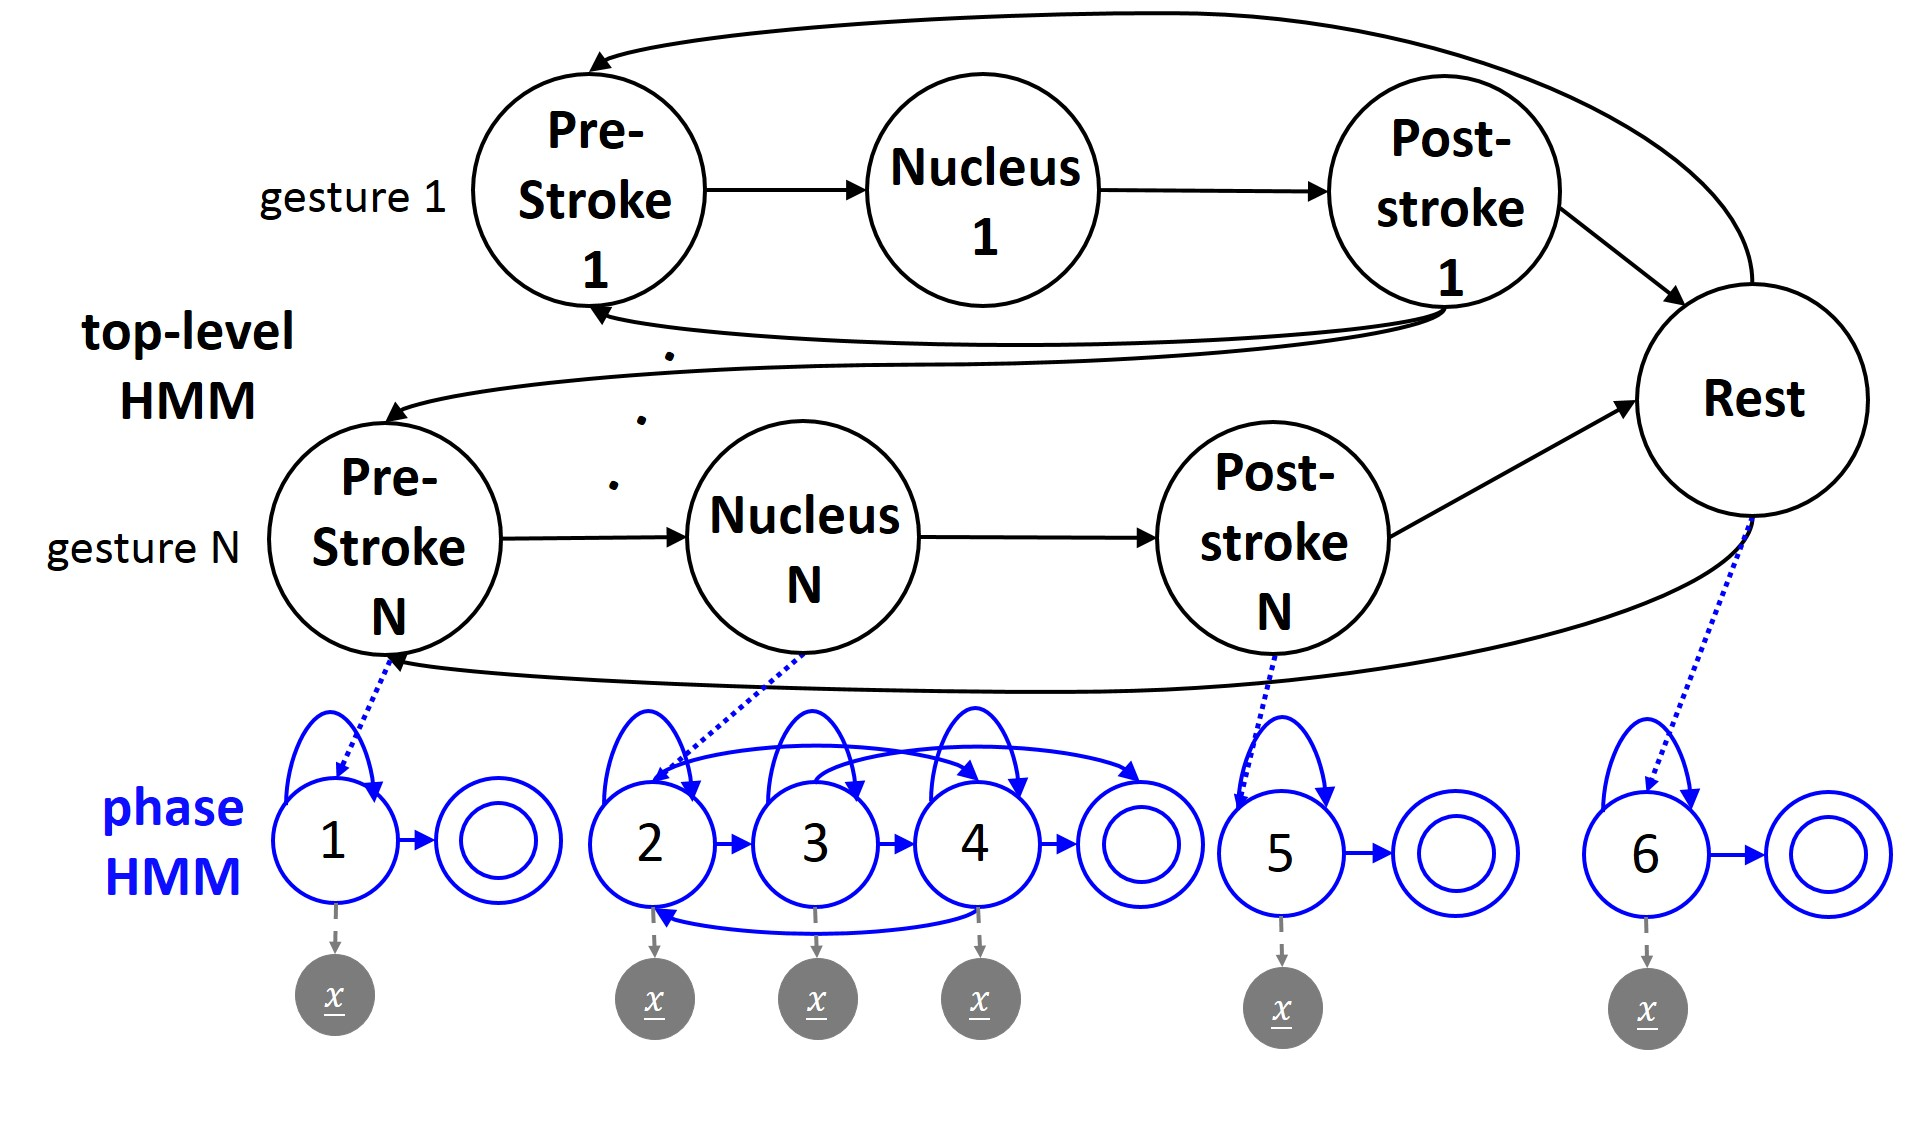
\includegraphics[width=\columnwidth]{figures/hhmm.jpg}
\caption{State transition diagram of the HHMM representation of the
gesturing process.
Solid arcs represent horizontal transitions between states; dotted arcs
represent vertical transitions, i.e., calling a phase HMM (sub-HMM).
Double-ringed states are end states. Only examples of transitions are shown
here.}
\label{fig:hhmm}
\end{figure}

The HHMM is an extension of the HMM that is designed to model domains with
hierarchical structure and/or dependencies at multiple length/time
scales~\cite{murphy02}. In an HHMM, the states of the stochastic automaton can
emit single observations or strings of observations. Those that emit single
observations are called ``production states'' (blue circles in
Figure~\ref{fig:hhmm}, and those that emit sequences of observations are termed
``abstract states'' (black circles). The abstract states call sub-HMMs to which
I refer as phase HMMs here.

We can represent the HHMM as a dynamic Bayesian network (DBN) (a
directed graphical model)~\cite{murphy02} as shown in Figure~\ref{fig:ahmm}.
The state of the whole HHMM at time $t$ is encoded by the vector $(G_t, P_t, S_t)$ where $G_t$ is the gesture label, $P_t$ is the
phase label, and $S_t$ is the hidden state representing a sub-stage in a
gesture phase. $F_t^d$ is a binary indicator variable that is
``on'' (has value 1) if the lower level HMM at time $t$ has just ``finished''
(i.e., is about to enter an end state), otherwise it is ``off'' (value 0).
The bottom level $X_t$ are the observations. 

\tikzstyle{vertex}=[circle, draw, minimum size=16pt, inner sep=0pt]
\tikzstyle{observed-vertex}=[circle, draw, minimum size=16pt, inner sep=0pt,
               fill=black!20] 
\tikzstyle{edge} = [draw, thick, -]
\tikzstyle{directed-edge} = [draw, thick, ->]

\begin{figure}[!tbh]
\centering
  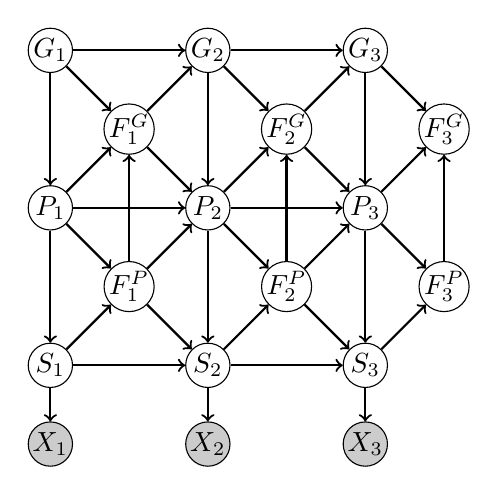
\begin{tikzpicture}[auto,swap, scale=2]
    % First we draw the vertices
    \foreach \pos/\name in {{(0, 2)/P_1}, {(1, 2)/P_2}, {(2,2)/P_3},
      {(0, 3)/G_1}, {(1, 3)/G_2}, {(2,3)/G_3},     
      {(0.5,2.5)/F_1^G}, {(1.5,2.5)/F_2^G}, {(2.5, 2.5)/F_3^G},
      {(0.5,1.5)/F_1^P}, {(1.5,1.5)/F_2^P}, {(2.5, 1.5)/F_3^P}, {(0, 1)/S_1},
      {(1, 1)/S_2}, {(2, 1)/S_3}} 
      \node[vertex] (\name) at \pos {$\name$};
    \foreach \pos/\name in {{(0, 0.5)/X_1}, {(1, 0.5)/X_2}, {(2, 0.5)/X_3}}
      \node[observed-vertex] (\name) at \pos {$\name$};
    % Connect vertices with edges and draw weights
    \foreach \source/ \dest in {P_1/S_1, S_1/X_1, P_1/F_1^P, S_1/F_1^P,
        G_1/P_1, G_2/P_2, G_3/P_3, G_1/G_2, G_2/G_3,
        G_1/F_1^G, G_2/F_2^G, G_3/F_3^G, P_1/F_1^G, P_2/F_2^G, P_3/F_3^G,
        F_1^G/G_2,  F_2^G/G_3, F_1^G/P_2, F_2^G/P_3, 
        F_1^P/F_1^G, F_2^P/F_2^G, F_3^P/F_3^G, 
        F_1^P/P_2, P_1/P_2, P_2/S_2, S_2/X_2, P_2/F_2^P,
        S_2/F_2^P, F_2^P/P_3, P_2/P_3, P_3/S_3, S_3/X_3,
        P_3/F_3^P, S_3/F_3^P, S_1/S_2, S_2/S_3,
        F_1^P/S_2, F_2^P/S_3} 
      \path[directed-edge] (\source) -- (\dest);
  \end{tikzpicture}
  \caption{DBN representation of the HHMM for the temporal gesture model. $G_t$ is the gesture label, $P_t$ is the
phase label, and $S_t$ is the hidden state representing a sub-stage in a
gesture phase. $F_t^d = 1$ if the HMM at the lower level has finished
(entered its exit state), otherwise $F_t^d = 0$. Shaded nodes are observed; the
remaining nodes are hidden.}
  \label{fig:ahmm}
\end{figure}

The $F_t^d$ binary indicator in the hierarchical model allows us to do
simultaneous segmentation and recognition. I want to avoid doing segmentation first and then find the most
likely HMM for the given sequence, because segmentation based on
differentiating rest position versus non-rest position will not allow the system
to respond fast enough. I want the system to respond at the beginning of the
post-stroke phase rather then at the beginning of the rest position. In
addition, making a hard decision on segmentation can introduce errors that
are hard to correct later. 

Even though the HHMM gives an appropriate model of temporal gestures,
performing exact inference on it can be slow due to the loops in the graphical
model (Figure~\ref{fig:ahmm}). To make possible a real-time system, I flatten
the hierarchical HMM into a one-level HMM for fast training and inference. This
is done by creating an HMM state for every leaf in the HHMM state transition
diagram (i.e., every legal HHMM stack configuration)~\cite{murphy02}, assuming that the states in the
phase-HMMs are not shared.
The effect of the $F_t^d$ binary indicator can be achieved by modeling the termination probability of each
state, $t(\text{END}|s)$, i.e., the probability for state $s$ to transit to the
end state in the phase HMM.

When flattening the HHMM, we need to add to the flattened model all the
transition probabilities among phase HMMs in the original hierarchal model. For example,
after flattening the HHMM in Figure~\ref{fig:hhmm}, we have (among others)
\begin{align*}
P_{flat}(5\rightarrow6) &= P_h(5\rightarrow \text{END} \rightarrow \text{Rest}
\rightarrow 6 )\\
P_{flat}(4\rightarrow5) &= P_h(4\rightarrow \text{END} \rightarrow 
\text{Post-stroke N} \rightarrow 5)
\end{align*}
where $P_h$ represents the probability in the HHMM.

Flattening the HHMM into an one-level HMM does have some disadvantages. First,
flattening loses modularity, since the parameters of the phase HMMs get
combined in a complex way~\cite{murphy02}. A separate index is needed
to map the hidden states back to the abstract states (the phase and gesture
labels) they correspond to. Secondly, training HMMs separately and combining
them together in one model requires segmented data, i.e., data about an
individual gesture.
However, getting separate training examples for different gestures is not a difficult task in this case. Lastly, an HHMM can represent and learn sub-models that are re-used in different contexts, but an HMM cannot do this~\cite{murphy02}.

\section{Unified Framework}
To include both path and pose gestures within the model, I use different
topologies for their corresponding phase HMMs because
they have different characteristics in terms of hand movement.

Based on the standard HMM\footnote{See Appendix~\ref{app:hmm} for more details
about the HMM.} formulation, the probability of a sequence of observation,
$\underline{x}_{1:T} = \underline{x}_1\ldots\underline{x}_T$, and the corresponding hidden states sequence, $s_{1:T} = s_1\ldots s_T$, is given by
\begin{align}
P(\underline{x}_{1:T}, s_{1:T};\underline{\theta}) = 
    t(s_1)t(\text{END}|s_T)\prod_{t = 2}^T t(s_t | s_{t-1})\prod_{t = 1}^T
    e(\underline{x}_t|s_t)\label{eq:hmm}
\end{align}
where $\underline{\theta}$ represents the model parameter vector which includes
the initial state probabilities $t(s)$, the state transition probabilities $t(s'|s)$, the 
emission probabilities $e(\underline{x}|s)$,
and the termination probabilities $t(\text{END}|s)$ for $s, s'\in \{1, 2,\ldots
H\}$. In this section, I describe how I model these conditional
probability distributions (CPDs), and compute the model parameters for both
path and pose gestures, combining them together under the unified HMM-based
framework. Note that the term ``unified framework'' means that the two forms of
gestures are combined under the same probabilistic framework, but there are
still differences in the models for the two gestures, e.g., different topologies
and different training strategies.

\subsection{Path Gestures}
If we have ground truth labels for the pre-stroke, the nucleus and the
post-stroke phases (as we do in the ChAirGest dataset), we can train the
phase HMMs for each phase and each gesture separately, then concatenate the
phase HMMs (i.e., the concatenated HMMs\footnote{See my previous
publication~\cite{yin13} for details.}).
However in practice, for example if we want users to be able to easily add their new gestures by giving a few
examples, it will be tedious to manually label the start and the end of the
three phases. In this case, I use embedded training \cite{young1994}, i.e.
train each phase HMM embedded in an entire gesture segment
(Figure~\ref{fig:embed}).

\begin{figure}[tbh]
\centering
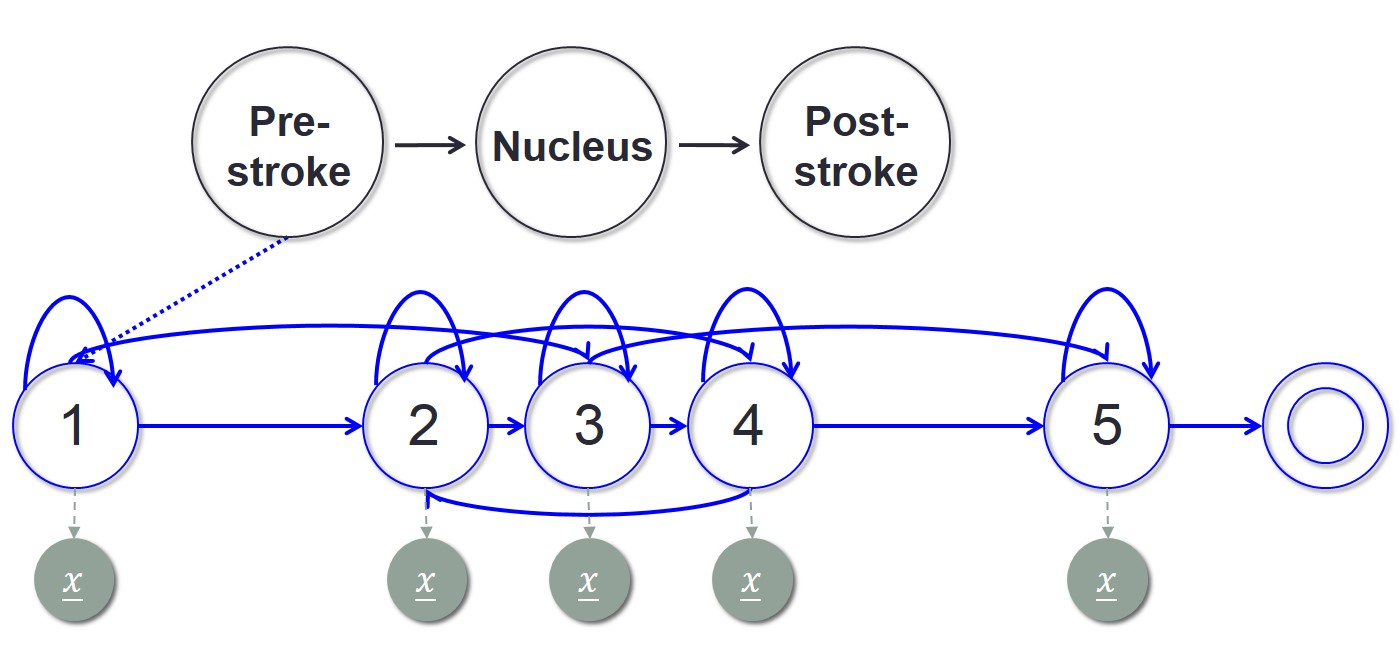
\includegraphics[width=0.7\columnwidth]{figures/embedded.jpg}
\caption{Embedding phase HMMs into an entire gesture.}
\label{fig:embed}
\end{figure}

With the YANG dataset, I choose to use one hidden state for pre-stroke and
post-stroke phases through cross-validation. I use the Bakis (left-right with
skips) topology~\cite{Bauer00} for the nucleus phase, but add a backward
transition from the last hidden state to the first one for gestures with an
arbitrary number of repetitions (e.g., the Wave gesture)
(Figure~\ref{fig:bakis}). The left-right topology not only closely models the temporal evolution of a gesture, it also reduces the model complexity
by constraining the number of possible transitions. Without this constraint,
the model would have $O(H^2)$ transition parameters; with the left-right
constraint, it only has $O(H)$ transition parameters where $H$ is the
number of hidden states in the HMM.

\tikzstyle{vertex}=[circle, draw, minimum size=16pt, inner sep=0pt]
\tikzstyle{observed-vertex}=[circle, draw, minimum size=16pt, inner
sep=0pt, fill=black!20] 
\tikzstyle{edge} = [draw, thick, -]
\tikzstyle{directed-edge} = [draw, ->]
\begin{figure}[!tbh]
\centering
  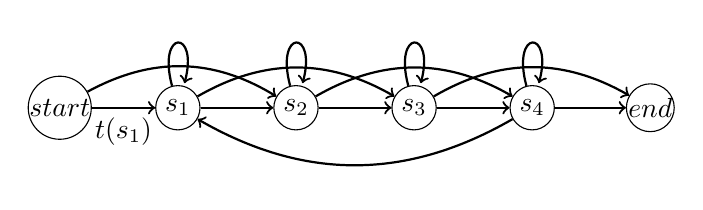
\begin{tikzpicture}[auto,swap, scale=1.5]
    % First we draw the vertices
    \foreach \pos/\name in {{(0, 0)/start}, {(1, 0)/s_1}, {(2, 0)/s_2},
    {(3, 0)/s_3}, {(4, 0)/s_4}, {(5, 0)/end}}
      \node[vertex] (\name) at \pos {$\name$};
    % Connect vertices with edges and draw weights
    \foreach \source/ \dest in {s_2/s_3, s_3/s_4, s_4/end,
    s_1/s_2} \path[directed-edge] (\source) -- (\dest);
    
    \foreach \source/ \dest in {s_1/s_3, start/s_2, s_2/s_4, s_3/end, s_4/s_1} 
      \path[directed-edge] (\source) edge [bend left] (\dest);
      
    \foreach \source/ \dest in {s_1/s_1, s_2/s_2, s_3/s_3, s_4/s_4} 
      \path[directed-edge] (\source) edge [loop above] (\dest);
    
    \path[directed-edge] (start) edge node [below] {$t(s_1)$} (s_1);
  \end{tikzpicture}
  \caption{A state transition diagram of a modified 4-state Bakis model for the nucleus phase.}
  \label{fig:bakis}
\end{figure}

In Chapter~\ref{chap:feature}, I showed that the features I use follow mixture
of Gaussians (MoG) distributions, hence I use MoG with diagonal covariances to
model the emission probability, i.e.,
\begin{align}
e(\underline{x} | s) = \sum_{m=1}^k q(m | s)\mathcal{N}(\underline{x};
\mu_{s,m}, \Sigma_{s, m})
\end{align}
where $k$ is the number of mixtures.
Figure~\ref{fig:mog} shows the DBN representation of an HMM of MoG emission
probabilities. The covariance, $\Sigma_{s, m}$, has a fixed prior of $0.01\times
I$ which is added to the maximum likelihood estimate to prevent the covariance from shrinking to a point/delta function. 

\begin{figure}[tbh]
\centering
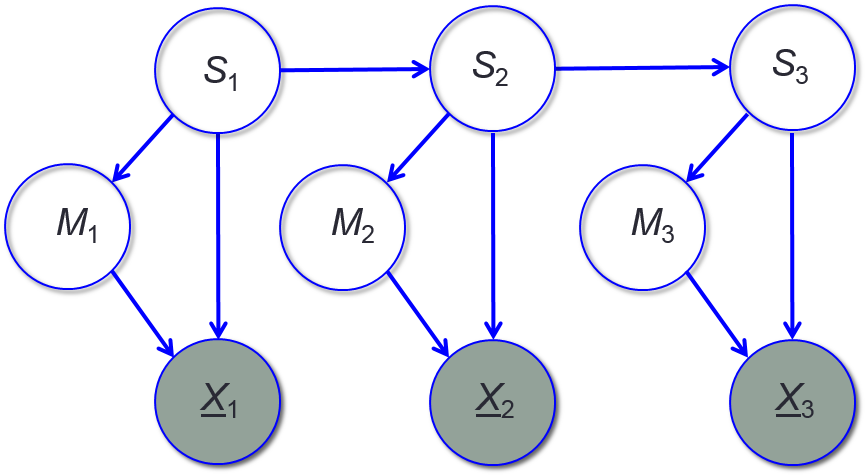
\includegraphics[width=0.5\columnwidth]{figures/mog.png}
\caption{DBN representation of HMM with mixture of
Gaussians emission probabilities.}
\label{fig:mog}
\end{figure}

\subsubsection{Training Strategies}
I use two-pass training to estimate the model parameters for each path
gesture HMM separately. Currently, training is done in MATLAB using Kevin
Murphy's HMM toolbox\footnote{\url{https://code.google.com/p/bnt/}}.

The first pass is Viterbi training\footnote{See Appendix~\ref{sec:viterbi} for
details}.
In this pass, only the pre-stroke hidden state can be the initial state and
only the post-stroke hidden state can be the termination
state. The emission probability parameters are initialized by dividing the data
sequence into $H$ segments of equal length (where $H$ is the total number of
hidden states in the embedded HMM) and associating each successive segment with
successive states~\cite{young1994}. For each segment, the K-means algorithm is used to initialize MoG parameters. In each iteration of the training, the most likely path is computed using the
Viterbi algorithm. For all the observations assigned to the same hidden
state, K-means algorithm is used again to find the new MoG parameters for
that state. The Viterbi training provides a better alignment of data with the
hidden states, and thus gives a better initialization of the MoG parameters. 

The second pass is Baum-Welch training that computes the maximum likelihood
estimate of the parameters.
It uses the estimated MoG parameters as the initial values. It also relaxes the
initial state probabilities (allowing the first two states to be the start
state) and the termination probabilities (allowing the last two states to be the
termination state). This allows the possibility of transitions between nucleus
phases without going through pre-strokes and post-strokes when we combine the
individual gesture HMMs together. For natural interaction, this is important
because sometimes users may do two gestures immediately after one another, with
no post-stroke. When initializing the transition matrix, all the allowed
transitions are set to the same value, so that no states are favored arbitrarily. Transitions that are not allowed are initialized to zero.

The Baum-Welch estimation formulae for MoG parameters and transition parameters
are well established. Here, I give the formula for the termination probability.
Given $N$ training sequences, the update for the termination probability during the $i$th iteration is 
\begin{displaymath}
t^i(\text{END}|s) = \frac{\sum_{j = 1}^N \overline{count}(j, s\rightarrow
END;\underline{\theta}^{i-1})} {\sum_{j = 1}^N\sum_{s'} \overline{count}(j, s\rightarrow s';\underline{\theta}^{i-1})}
\end{displaymath}
where $\overline{count}(j, s\rightarrow END;\underline{\theta}^{i-1})$ is the expected count of 
$s$ being the end state. We can use the usual forward-backward algorithm to compute all the 
expected sufficient statistics by adding a dummy END state to the end of each
sequence (see Appendix~\ref{sec:term} for details).

\subsection{Pose Gestures}
I use one hidden state, $s_{\text{pose}}$, to represent of the nucleus phase of
a pose gesture (Figure~\ref{fig:single}). Within a user,
there may be variation in the hand pose used for a particular pose gesture.
For example, the Point hand pose can have different orientations.
Hence, I also use the MoG for the emission probability
$e(\underline{x} | s_\text{pose})$. 

\begin{figure}[tbh]
\centering
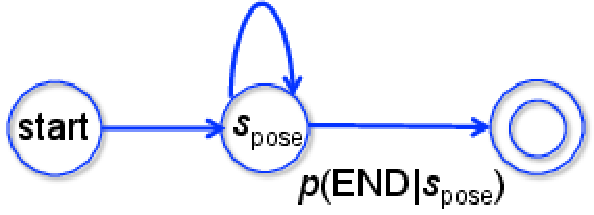
\includegraphics[width=0.5\columnwidth]{figures/single_state.pdf}
\caption{State transition diagram of a single state HMM for gestures with
distinct hand poses. }
\label{fig:single}
\end{figure}

The number of mixtures for pose gestures are greater than that of path
gestures, made to capture the variation in hand poses people use. The number
of mixtures can also be different for different pose gestures.
This is because some hand poses may have more variation than others.
For example, the Point gesture may have more variations in orientations than
Grab gesture (hand in fist).

\subsubsection{Training Strategies}\label{sec:pose-gesture}
Because there is only
one hidden state, I directly compute the maximum likelihood estimates of the MoG
parameters for emission probability of $s_{\text{pose}}$ using an
expectation--maximization (EM) algorithm, instead of doing embedded training.

The number of mixtures is
determined using the Bayesian Information Criterion (BIC)~\cite{fraley06}:
\begin{align*}
\text{BIC}\eqdef2\text{loglik}(\underline{x}_{1:n}, \underline{\theta}_k^*) -
(\text{\# params})\log(n)
\end{align*}
where $\text{loglik}(\underline{x}_{1:n}, \underline{\theta}_k^*)$ is the
maximized loglikelihood for the data and the model with $k$ mixtures per state, (\# params) is the number of independent parameters to be estimated in the model, and $n$ is the number of observations in
the data. Let $d$ be the feature vector dimension, then $\mu_{s,m}$ for
hidden state $s$ and mixture $m$ has $d$ independent parameters, and the
diagonal covariance matrix $\Sigma_{s,m}$ has $d$ independent parameters as
well. Because $\sum_{m=1}^k q(m | s) = 1$, the number of independent parameters
for the weights $q(m|s)$ is $k - 1$. Hence,(\# params) is computed as:
\begin{align*}
\text{\# params} = (k - 1) + (d + d) * k
\end{align*}
The $k$ that gives the highest BIC is chosen from a predetermined range
(determined through cross-validation).

For each $k$, Expectation Maximization (EM) is used to estimate the means,
covariance matrices and mixture probabilities of the MoG. As the EM algorithm may
converge to a local optimum of the observed data likelihood~\cite{dicintio12}, I
repeat the optimization 3 times using K-means algorithm with random
initialization to set the initial cluster centers, and choose the model that
gives the maximum likelihood.

The training data for pose gestures should contain random variations in the
hand movement so that the resultant variances for the motion features will be
larger, making motion features less important in
$e(\underline{x}|s_{\text{pose}})$. Figure~\ref{fig:covariance} gives an
illustration of this by comparing two covariance matrices of the MoG for hidden
states from two \textit{forms} of gestures.
The variance values are normalized between the two matrices for each feature to make
them comparable. We can see that the variances for the motion features (features
1--9) are larger (with darker colors) for the pose gesture.

\begin{figure}[tbh]
\centering
\subfigure[Covariance of a MoG of a path gesture.]{
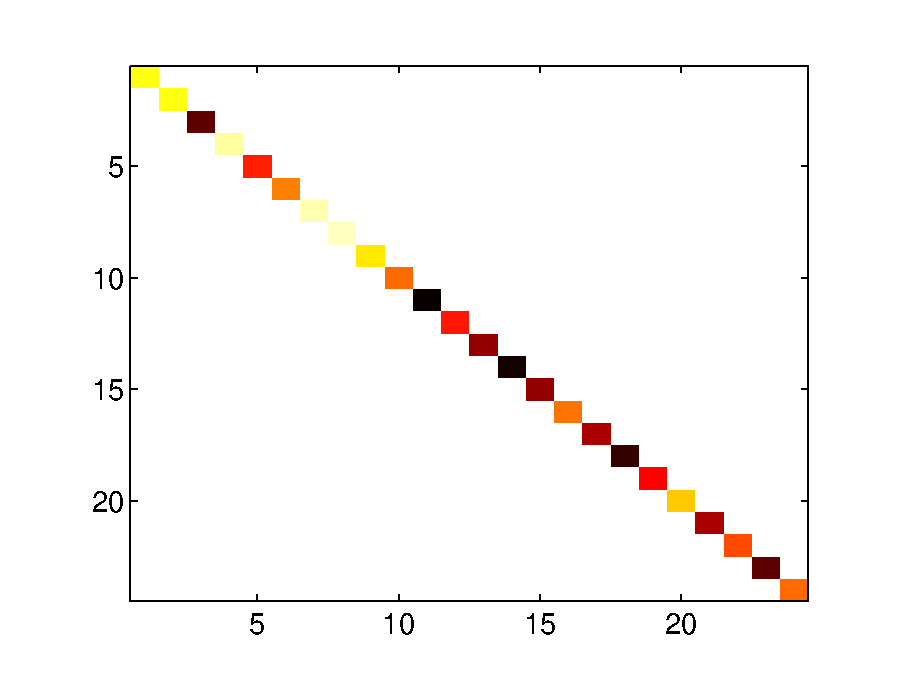
\includegraphics[trim=1.3cm 0 1cm
0.5cm, clip, width=0.45\columnwidth]{figures/covariance_path.eps} }
\subfigure[Covariance of a MoG of a pose gesture.]{
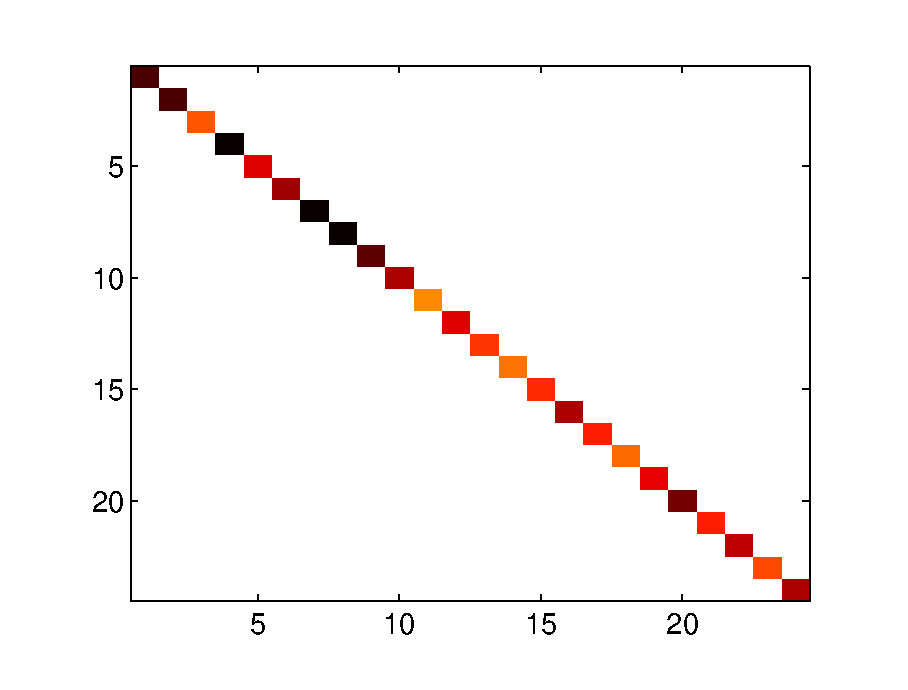
\includegraphics[trim=1.3cm 0
1cm 0.5cm, clip, width=0.45\columnwidth]{figures/covariance_pose.eps} }
\caption{Visualization of normalized covariance matrices of the MoG for
different hidden states. The darker the color, the larger the variance.}
\label{fig:covariance}
\end{figure}

It is possible that a gesture with a distinct path also has the same hand pose
as another gesture with distinct hand pose, for instance, some user may prefer
to do the Circle gesture with their hand in a point hand pose. In this case, the
gesture will be recognized as the Circle gesture because the Circle gesture
model matches both the hand pose and the path and thus will 
have a higher likelihood after considering a few consecutive frames.

Since there is only one hidden state for $s_{\text{pose}}$, its transition
probability is 1. Its termination probability is estimated according to the
expected duration of the gesture. The self-arc on a state in an HMM defines a 
geometric distribution over waiting time \cite{murphy02}. In the case of a
single state HMM, the probability of remaining in state $s_{\text{pose}}$ for
exactly $d$ steps is $P(d) = p(1-p)^{d - 1}$, where $p = P(END|s_\text{pose})$
is the termination probability for $s_{\text{pose}}$. This means the expected
number of steps remaining in state $s_{\text{pose}}$ is $\frac{1}{p}$. I assume
that the minimum duration of a path gesture is one
second (30 frames). The termination probability $P(END|s_\text{pose})$ is then set to
be less than $\frac{1}{30}$.

I use one hidden state to model the rest position in a similar way.

\section{Real-time Gesture Recognition}
I train one HMM, $\underline{\theta}_g$, for each gesture (path or pose) $g\in
\{1\ldots G\}$, then combine them into a one-level HMM flattened from the HHMM
in Figure~\ref{fig:hhmm}, assuming uniform transition probabilities among
gestures.

\subsection{Combined HMM}\label{sec:combined}
I use a superscript $c$ to denote the model
parameters in the combined HMM. Let $H_{g}$ be the number of hidden states for
gesture $g$. The total number of hidden states in the combined HMM, $H^c$, is then
\begin{align*}
H^c = \sum_g H_{g}
\end{align*}
The model for each path gesture starts with a hidden state for the pre-stroke,
then 1 or 2 hidden states for the nucleus, followed by a hidden state for the
post-stroke. Each pose gesture has a hidden state for the nucleus. The combined
HMM has a sequential labeling for these hidden states, with the hidden state label for the pre-stroke of the second gesture model following
the hidden state label for the post-stroke of the previous gesture, etc.
Formally, the new hidden states labels are in $\{1\ldots H^c\}$, and
the hidden states from $(\text{base}_i + 1)$ to $(\text{base}_g + H_{g})$
belongs to gesture $g$ where $base_g$ is the base index
\begin{align*}
\text{base}_g = \sum_{j=1}^{g-1}H_{j}
\end{align*}
Figure~\ref{fig:combined-hmm} gives an example of the labeling scheme in
the combined HMM. This scheme allows an easy mapping of hidden state labels
back to their corresponding gestures and phases.

\begin{figure}[!tbh]
\centering
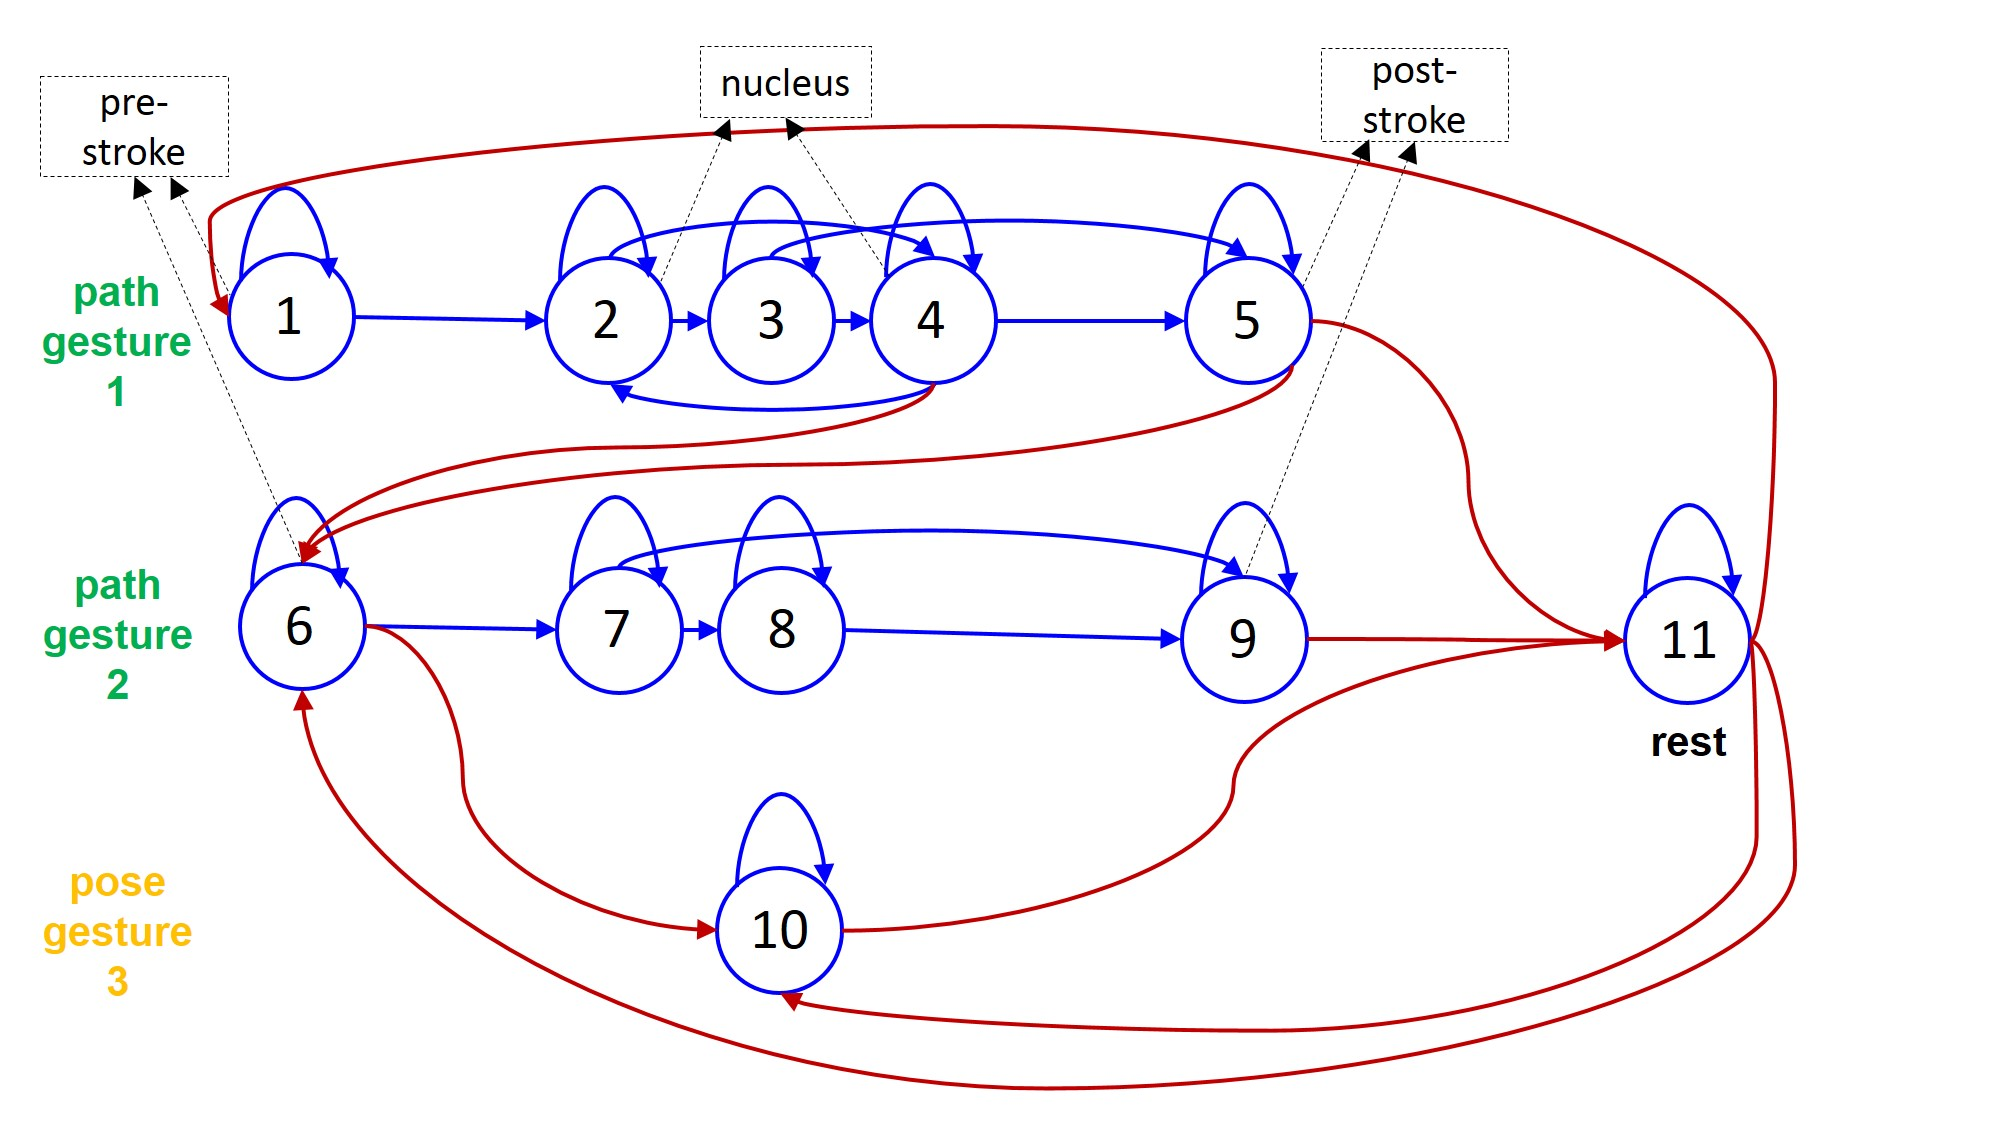
\includegraphics[width=\columnwidth]{figures/combined_hmm.jpg}
\caption{Combined HMM. The red lines are examples of transitions added to
combine the individual gesture HMMs.
To keep the diagram from getting cluttered, not all possible transitions are shown.}
\label{fig:combined-hmm}
\end{figure}

The non-trivial part in creating the combined HMM is computing the new 
transition probabilities. The initial state probability in the combined
HMM, $t^c(s)$, for $s\in\{1\ldots H^c\}$ is
\begin{align*}
t^c(s) = \frac{t(s)}{\sum_{s'=1}^{H^c} t(s')}
\end{align*}
The probability of an $s$ to $s'$ transition
in the combined model is the sum over all paths from $s$ to
$s'$ for $s, s'\in\{1\ldots H^c\}$~\cite{murphy02}. In our model, 
\begin{align}
t^c(s'|s) = t(s' | s) (1-t(\text{END}|s)) +
t(\text{END}|s)t^c(s')
\label{eq:combined-transition}
\end{align}
where $t(s'|s)$ is the transition probability in the individual gesture HMM if
$s$ and $s'$ are from the same gesture; otherwise it is zero. Note that
$t(s'|s)$ is normalized such that $\sum_{s'}t(s'|s) = 1$ without taking into
account the termination probability $t(\text{END}|s)$ (as the end state is not
an actual hidden state), hence it is necessary to multiply $t(s'|s)$ by $
(1-t(\text{END}|s))$ in Equation~\ref{eq:combined-transition} to get the actual
unnormalized probability.

As the pre-strokes and post-strokes for different gestures can be similar, I
allow sharing of the pre-stroke hidden states and post-stroke hidden states
among gestures by adding a small transition probability (0.01) prior among
pre-stroke hidden states and among post-stroke hidden states (e.g.,
$t(s_{\text{pre-stroke}_i} | s_{\text{pre-stroke}_j}) = 0.01$).
Pose gestures also share the pre-stroke and post-stroke hidden states of path
gestures. The sharing of hidden states is similar to the mechanism of parameter
tying/sharing which is often used in speech recognition to improve the
robustness of the model when training data is limited~\cite{young1994}. Note
that these probabilities are not learned because the phase HMMs are trained
separately and the inability to learn shared structures is a disadvantage of
flattening the HHMM as mentioned earlier.

Finally, we need to make sure that the new transition matrix is stochastic,
i.e., 
\begin{align*}
\sum_{s' = 1}^{H^c} t^c(s'|s) = 1
\end{align*}
by normalizing $t^c(s'|s)$.

\subsection{Online Inference}
Once we have a combined model, I use fixed-lag smoothing \cite{murphy02} to do
online inference on the flattened HMM for real-time gesture recognition.
Fixed-lag smoothing is a modified forward-backward algorithm. Unlike online
filtering, which estimates the belief state at current time $t$ using
only a forward pass, we estimate the state at $t - l$, given all the
evidence up to the current time $t$, i.e., compute $\gamma_{t - l}(s) \eqdef P(S_{t -
l} = s|\underline{x}_{1:t})$, where $l > 0$ is the lag (see
Figure~\ref{fig:inference}).
Introducing lag time is a tradeoff between accuracy and responsiveness. Using some future evidence to
smooth the estimate can increase the accuracy while adding some delay. However
if the delay is small, it might be unnoticeable.
In the Experiment Evaluation section (Section~\ref{sec:evaluation}), I show
details about the relationship between $l$ and the recognition performance.

\begin{figure}[tbh]
\centering
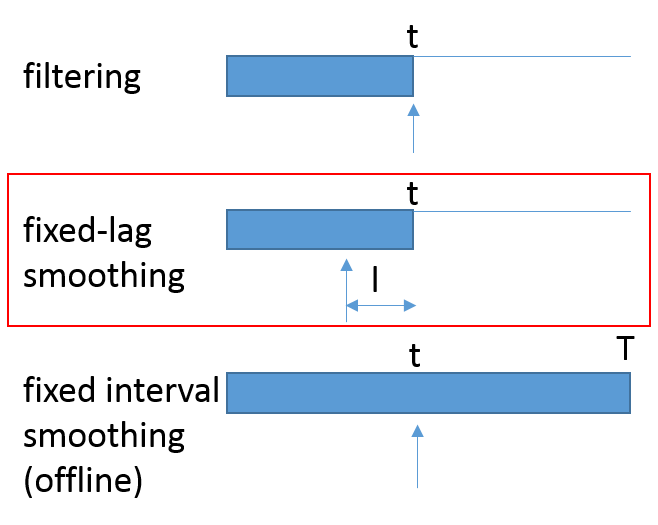
\includegraphics[width=0.5\columnwidth]{figures/inference.png}
\caption{Figure adapted from~\cite{murphy02} comparing different kinds of
inference. The shaded region is the interval for which we have data. The arrow
represents the time step at which we want to perform inference. $t$ is the
current time, and $T$ is the sequence length (see Appendix~\ref{sec:inference}
for details).}
\label{fig:inference}
\end{figure}

Fixed-lag smoothing can be implemented efficiently. I compute forward
probabilities $\alpha_t(s) \eqdef P(S_t = s|\underline{x}_{1:t})$
normally\footnote{It is more common (see e.g.,~\cite{Rabiner90}) to define
$\alpha_t(s) = P(S_t = s, \underline{x}_{1:t})$; the difference is discussed in
Appendix~\ref{sec:hmm-infernece}.} and keep a history window of
$\alpha_{t - l}\ldots\alpha_t$.
At every time frame $t$, I compute backward probabilities
$\beta_{t-l'}(s)\eqdef P(\underline{x}_{t-l'+1:t}|S_{t-l'}=s)$ from the current time $t$ to $t - l$,
i.e., from $l' = 0$ to $l$. The base case is 
\begin{align}
\beta_t(s) = 1
\end{align}
Then $\gamma$ can be computed as
\begin{align}
\gamma_{t - l} \eqdef P(S_{t-l}=s|\underline{x}_{1:t}) \propto \alpha_{t -
l}\cdot\beta_{t - l}
\end{align}  
The time complexity at each time frame is $O((H^c)^2l)$. Note that at time $t$,
the belief state at $t - l$ is committed, while the belief state from $t - l + 1$ to $t$
will still be revised later. The space complexity is $O(H^cl)$ mainly for
storing a window of $\alpha_{t-1}\ldots\alpha_{t}$.

We can then compute the most likely hidden state at $t - l$:
\begin{align}
\hat{s} = \arg\max_s \gamma_{t - l}(s)
\end{align}
The most likely hidden state is then mapped to the gesture label it
belongs to (including the rest position) and the gesture phase. 

Gesture events are detected at the boundary of a phase change: start pre-stroke,
start gesture nucleus and start post-stroke. In this way
we achieve simultaneous segmentation and recognition. The gesture event
information, together with the gesture label for the nucleus phase, are sent to the application level.
The system achieves real-time performance at 30FPS on a consumer level machine
with a Intel Core2 Quad CPU (2.83GHz) and 8GB of memory.

\begin{figure}[t]
\centering
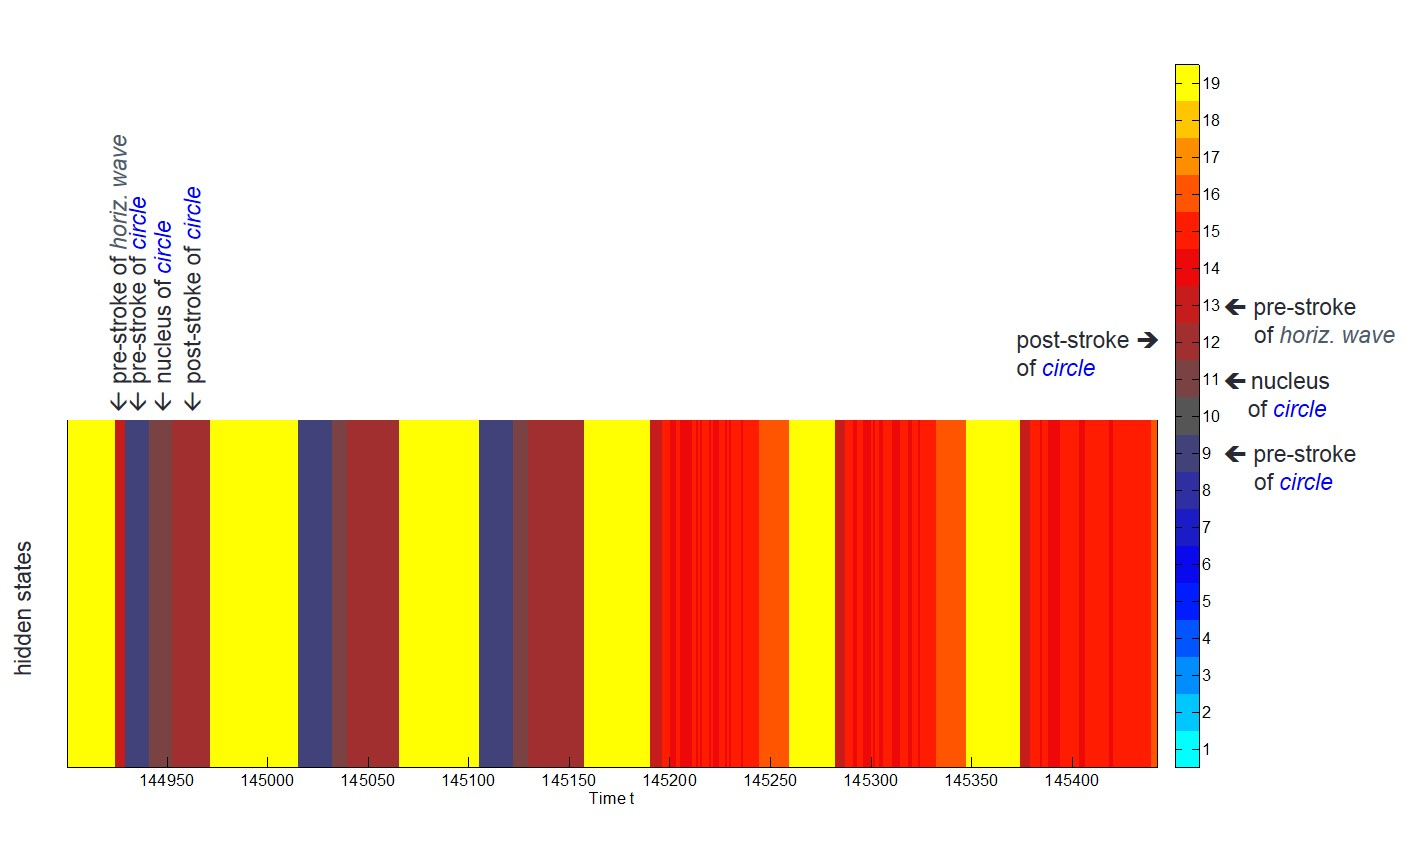
\includegraphics[trim=0 0 0
5mm, clip, width=\columnwidth]{figures/hidden_labeled.jpg}
\caption{Most likely hidden states using fixed-lag smoothing from a segment of
an input sequence.
Different colors indicate different hidden states. Yellow indicates rest position.}
\label{fig:visual_hidden}
\end{figure}

Figure~\ref{fig:visual_hidden} shows a visualization of the
most likely hidden states based on online fixed-lag smoothing inference
with $l = 5$ on a test sequence from the YANG dataset (only a segment is shown).
Notice that at the beginning of the hand movement, the most likely hidden state
is the pre-stroke for Horizontal Wave, but since a response is not required at this
time, the wrong estimate does not matter. After a few more frames, the estimates are
updated to have the correct most likely gesture label and the system
responds correctly when it detects the start of the post-stroke of the Circle
gesture.

\section{Gesture Spotting}
Identifying gesture phases allows us to distinguish gestures from non-gestures.
As every gesture must have a nucleus, any hand movement that does not have a
nucleus phase can be classified as a non-gesture. 

For example, when performing offline recognition, I use
MoG models for rest and non-rest positions to find non-rest segments (i.e.,
segments with hand movement), and for a non-rest segment, use
the Viterbi algorithm to find the most probable hidden state sequence $\hat{s}_1\ldots\hat{s}_T$ using
the mostly likely gesture model $\underline{\theta}_{\hat{g}}$
(see~\cite{yin13} for details).
Again, each hidden state can by classified into a pre-stroke
($s_\text{pre-stroke}$), nucleus ($s_\text{nucleus}$), or post-stroke
($s_\text{post-stroke}$) state.
The start and the end time for a gesture nucleus are the first and the last time
frame $t$ where $\hat{s}_t\in s_{\text{nucleus}}$ respectively. 

\begin{figure}[!tbh]
\centering
\subfigure[Gesture label result.
The pre-stroke and post-stroke phases are indicated by two orange colors (see the color bar).]{
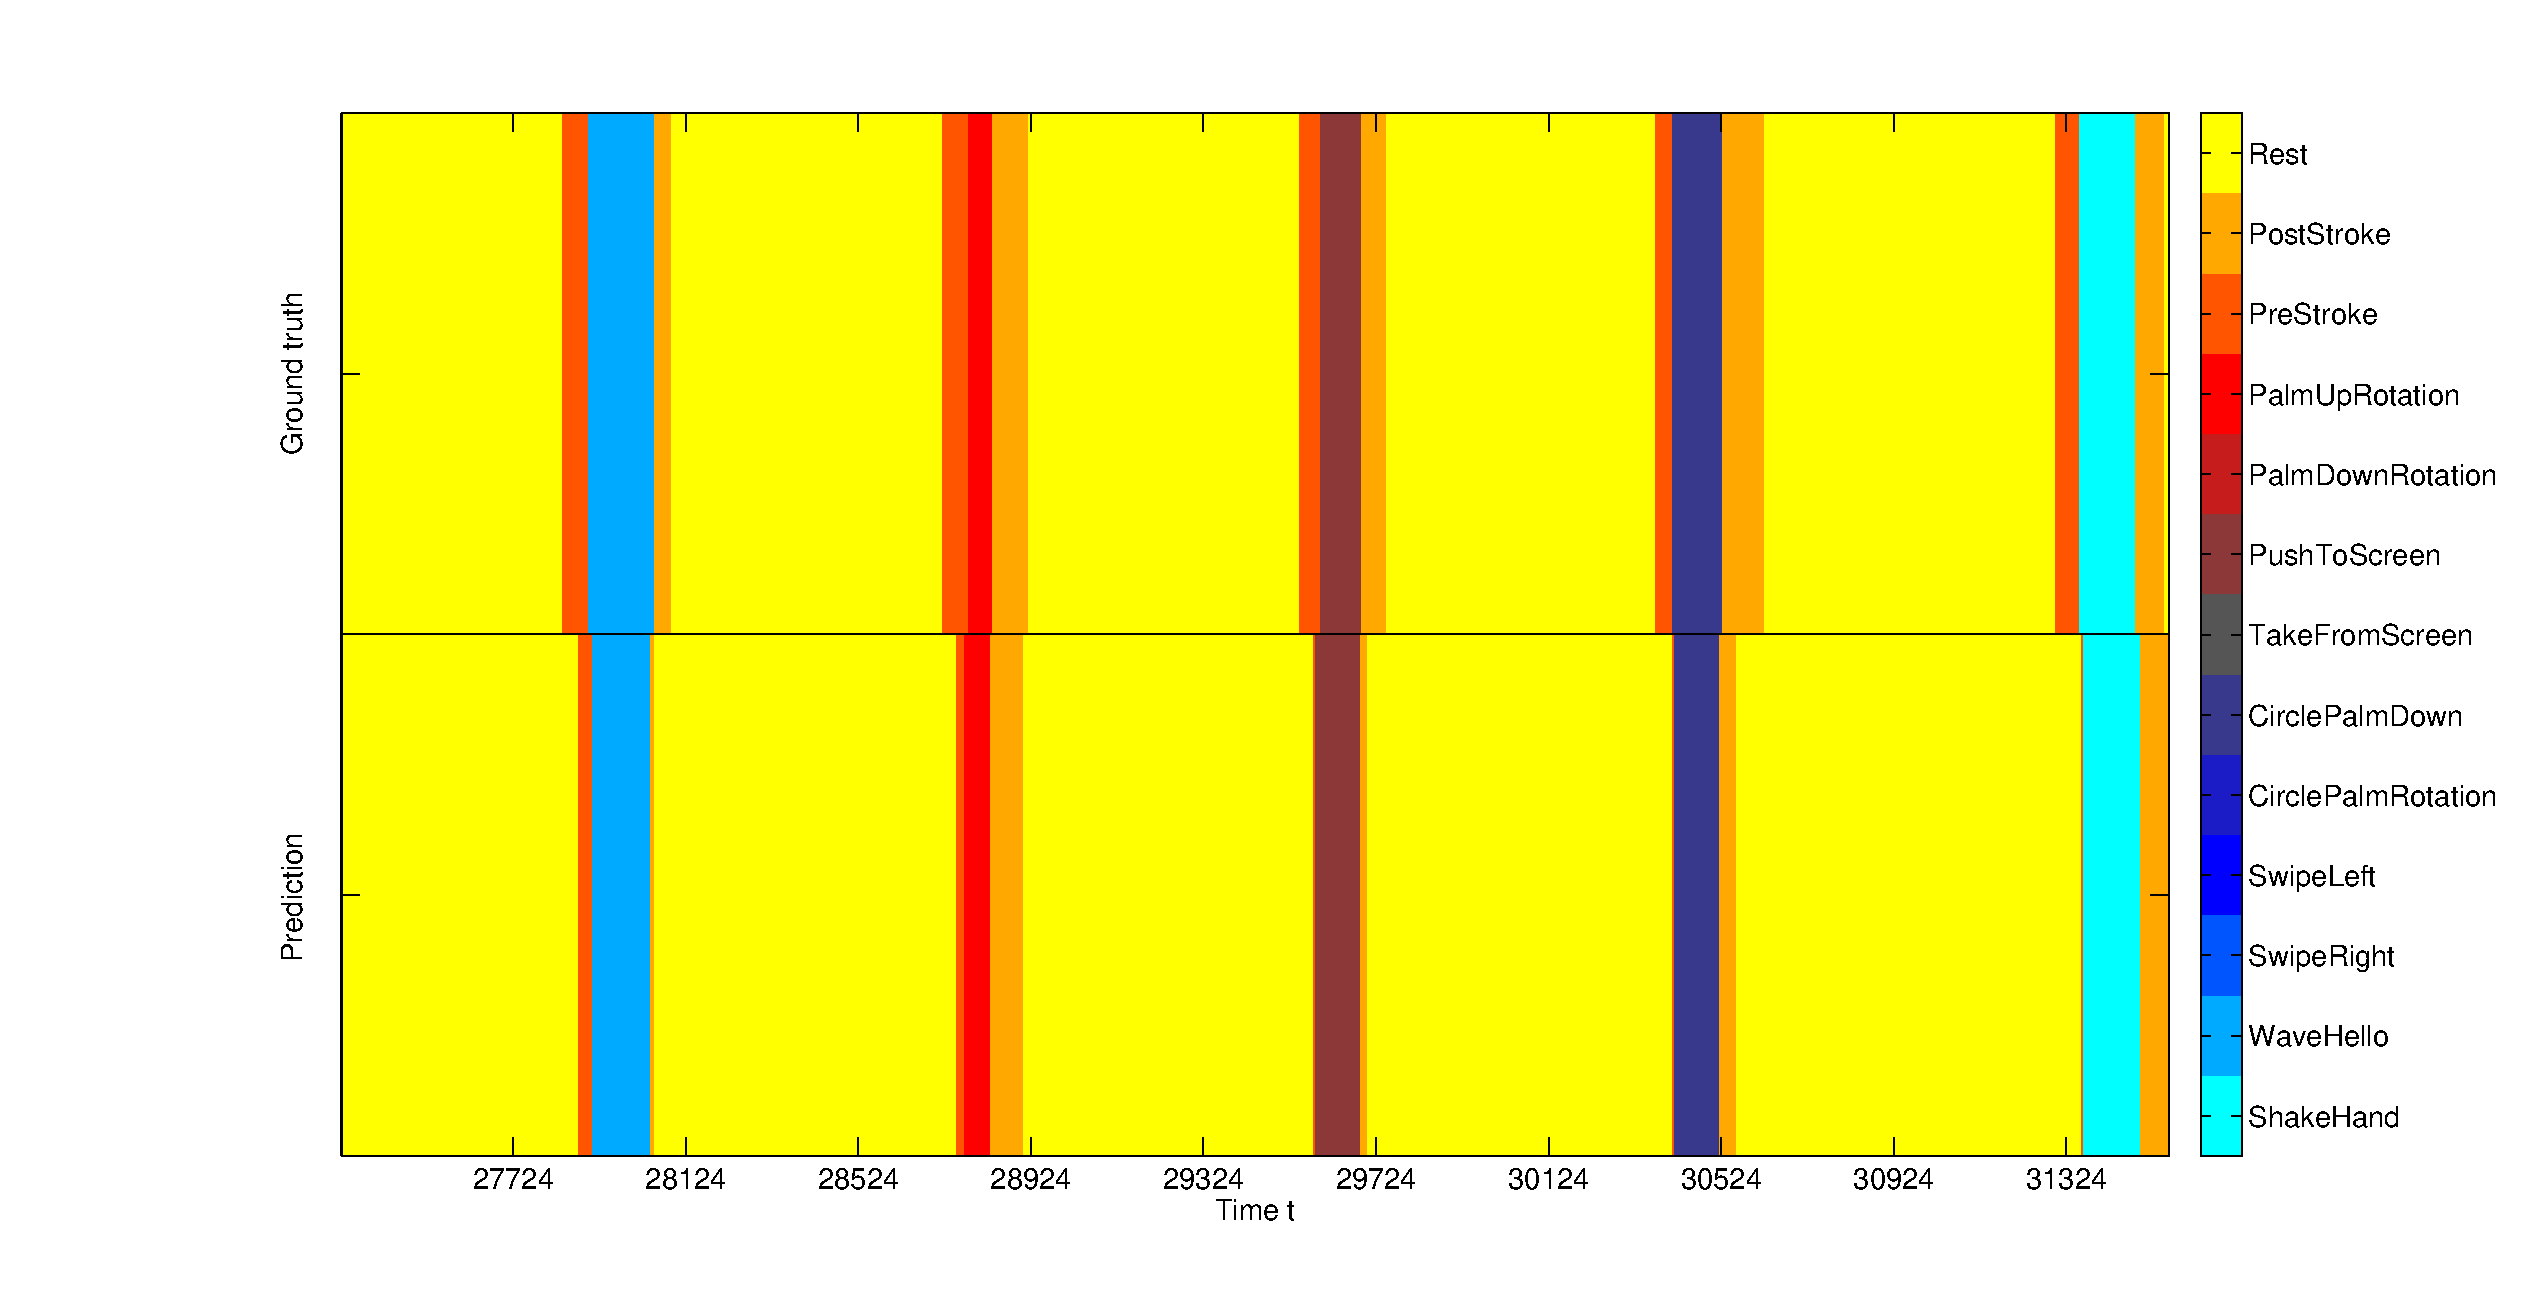
\includegraphics[trim={4cm 1cm 0cm 0.6cm}, clip,
width=1\columnwidth]{figures/gesture.eps}\label{fig:gesture-label}
}
\subfigure[Most probable hidden states.
Colors 1-3 indicate the pre-stroke hidden states, colors 4 - 9
indicate the nucleus hidden states, colors 10 - 12 indicate the post-stroke
hidden states, and color 14 indicates the rest state.]{
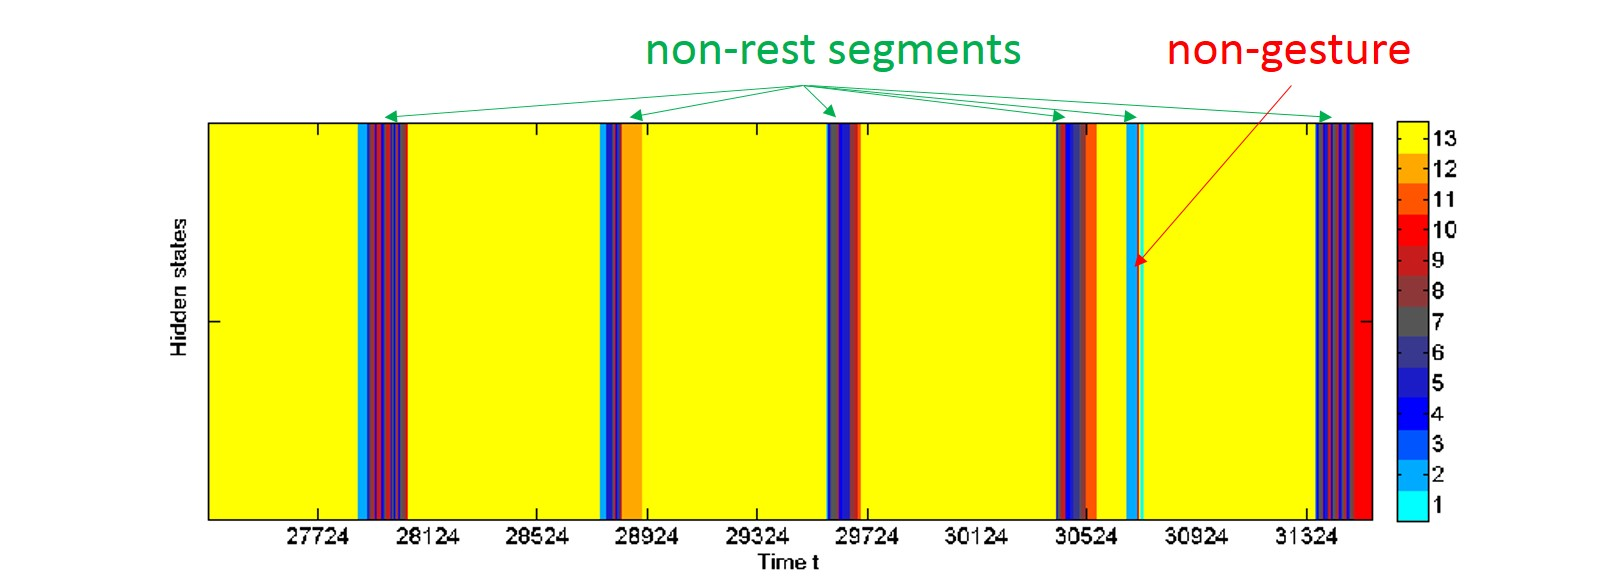
\includegraphics[trim={2.5cm 0cm 0.2cm 0cm}, clip,
width=1\columnwidth]{figures/hiddenstates_labeled.jpg} \label{fig:hiddenstates}
}
\caption{Visualization of gesture recognition result. A non-rest segment
without a nucleus phase (see $t\sim 30700$ in \subref{fig:hiddenstates}) is not
identified as a gesture (no label reported at the same time in
\subref{fig:gesture-label}.}
\end{figure}

Figure~\ref{fig:gesture-label} shows the recognition result for
one test sequence. The top row is the ground truth, with different colors
indicating different gesture phases or the rest position.
The second row is my segmentation and recognition result.
Figure~\ref{fig:hiddenstates} shows the color-coded most probable hidden states
for the same sequence.
If a non-rest segment does not contain hidden states belonging to the nucleus
phase, it is ignored (see the blue bar at $t\sim 30700$ in Figure~\ref{fig:hiddenstates}).
In this way, we can spot the actual gestures while filtering out other movements.

Using a thresholding method on the loglikelihood of a
given segment may not be robust, because the maximum loglikelihood of a
non-gesture segment among all gesture HMMs can be greater than that of a gesture segment.
The HMM formulation (Equation~\ref{eq:hmm}) implies that the longer the sequence the smaller the
likelihood (and hence the loglikelihood) because there are more probability
terms which are all smaller than 1 in the product terms. For example, the
loglikelihood of the fifth non-rest segment (a non-gesture) in
Figure~\ref{fig:hiddenstates} has a maximum loglikelihood of -296.6, while the
first non-rest segment (a gesture) has a maximum loglikelihood of -785.6. 
Even if we normalize the loglikelihoods by the segment lengths, the normalized
loglikelihood for the non-gesture (-14.8) is still greater than that of the
gesture (-17.9). As non-gestures are often shorter than gesture sequences, it
would hard to set a good threshold.
 
My gesture phase based method can be used in addition to a thresholding method
with a relative conservative threshold, i.e., a threshold that may cause false
positives but no false negatives so that the gesture phase based method can be used to further
filter out false positives.

\section{Concatenated HMM versus LDCRF}
Morency et al. formulated LDCRF~\cite{morency07} (an extension to CRF), and used
it for head and eye gesture recognition. In contrast to HMM (a
generative model), LDCRF is a discriminative model. It gives
per frame classification, and hence, can 
be used to do simultaneous segmentation and labeling. I applied LDCRF to gesture phase segmentation and recognition, and
compared the result with my concatenated HMM method~\cite{yin13}. 

As LDCRF requires per frame labeled training data, we need ground truth labeling
for the gesture phases. Hence, I use the ChAirGest dataset for this
evaluation. For all the non-rest segments in the training set, the nucleus
frames are labeled 1 -- 10 according to their corresponding gesture labels.
All the pre-stroke frames are labeled 11, and all the post-stroke
frames are labeled 12. This means the pre-strokes of all the gestures share the
same hidden states, and same for post-strokes. Using different hidden states
for pre-strokes and post-strokes of different gestures would increase
computation time significantly since it increases quadratically with the number
of hidden states (see Appendix~\ref{sec:linear-crf}). For each label, 6 hidden
states are used, resulting in 72 hidden states in total.

During testing, frames from the non-rest segments are classified into gesture
nucleus labels, pre-stroke or post-stroke using the trained LDCRF model. Using
the pre-stroke and post-stroke labels, we can find the start and end of the
nucleus phases. The HCRF
library\footnote{\url{http://sourceforge.net/projects/hcrf/}} which contains an implementation of the LDCRF model is used for both training and testing.

Table~\ref{tab:ldcrf} shows a comparison of the results between
using LDCRF and concatenated HMMs. The $F_1$ score of the concatenated HMMs
model is 7.7 percentage points higher than the LDCRF
model.
However, the LDCRF gives a slightly higher (1.5\%) temporal segmentation score,
ATSR.
Overall, the concatenated HMMs gives better performance (6.0\% higher) and,
importantly, takes 150 times shorter time to train (two orders of
magnitude).

\begin{table}[tbh]
\centering
\begin{tabular}{|l|l|l|}
\hline
& \thead{LDCRF} & \thead{Concatenated HMMs} \\
\hline
$F_1$ Score & 0.82 (0.03) & \textbf{0.897 (0.03)} \\
\hline
ATSR Score & \textbf{0.923 (0.02)} & 0.907 (0.02) \\
\hline
Final Score & 0.84 (0.02) & \textbf{0.90 (0.02)} \\
\hline
Training Time & 18hr & \textbf{7min} \\
\hline
\end{tabular}
\caption{Comparison of recognition results between LDCRF and concatenated
HMMs using the ChAirGest dataset.}
\label{tab:ldcrf}
\end{table}

\subsection{LDCRF Optimization}
One reason that LDCRF is so slow is that it considers all pair-wise transitions
among all the hidden states in the optimization process ($72^2$ transition
features in this case). However, since the hidden states are not shared among
gestures, we do not need to consider the transitions between hidden states
from different gestures. In order to decrease the training time, I reduce the
time complexity of the model by constraining allowed transitions among hidden states.

In HMM, we can specify the topology by initializing transitions that are not
allowed to zero. In LDCRF, I do the same by setting transitions that are not
allowed to always be zero (or negative infinity if loglikelihood is used) in
each update. The edge features only include allowed transitions as well,
reducing the number of features in the model needs to be optimized. A 
mask matrix is used to specify allowed transitions, and I call this masked
LDCRF. Using this optimization, I am able to reduce the training time to 11hr,
but this still means that LDCRF takes 100 times longer to train.

